%    Author: David Riser, University of Connecticut
%    File: thesis/chapters/inclusive.tex
%
%    Change Log:
%    -----------
%    - 2018/09/18: Document created using content from chapters/sidis.tex. 
%    - 2018/12/03: Adding new plots and increasing the quality of the content.  Trying to finalize documet by filling out sections.

\chapter{Inclusive Cross Section}

One of the primary goals of this thesis work is the accurate determination of cross sections for charged $\pi$ mesons in SIDIS.  The measurement of a cross section for a well known process such as elastic scattering or inclusive electron scattering is typically calculated (using the same data) before new cross sections are provided.  Not only does this procedure provide validation of the integrated luminosity factor, it also builds confidence that the overall quality of the dataset is high, the electron identification is accurate, and the list of files used in the analysis is reasonable.  In this chapter, the inclusive electron scattering cross section is discussed.  \\

\section{Motivation}
Inclusive electron scattering is the process $e p \rightarrow e X$, where only the final state electron is detected and the rest of the event is not (anything apart from the electron that is detected is not analyzed).  As a function of $W$ (the invariant mass of the final state ($\gamma^* + p$) system) the region below 2 GeV contains resonances and is often referred to as the resonance region.  Resonance structures are difficult to detect higher than about 2 GeV, and this region is typically called the \textit{deeply inelastic} region.  While the deeply inelastic region is used extensively for measurements in nuclear/particle physics, the goal of luminosity verification is achieved here by studying the resonance region.  This is due principally to the excess of Bethe-Heitler events which collect in the $2 < W < 3$ region for $E_{beam} = 5.498$ (such events are difficult to remove when detecting only the final state electron). \\

Measurement of the inclusive cross section is performed for each sector independently by counting reconstructed events $N_i$ in each bin $i$ of the phase space of $W$ and $Q^2$.  Experimentally the cross section for bin $i$ is, 

\begin{equation}
	\frac{d\sigma_i}{dW \; dQ^2} = \frac{N_i}{\mathcal{L} A_i B_i R_i} \frac{1}{\Delta W \; \Delta Q^2}
\end{equation}

where the factor $\mathcal{L}$ is the integrated luminosity for the time period over which the events $N$ were collected.  The correction factors $A_i$, $B_i$, and $R_i$ refer to the acceptance, bin center, and radiative corrections for bin $i$ respectively.  

\section{Inelastic Scattering Model}
A particularly important aspect of this validation study is the reference model.  Not only is the model used to predict the cross section for comparison, it is also sampled in the Monte Carlo event generators used in study detector acceptances and radiative corrections.  The model which is used in this study was first developed by Cynthia Keppel \cite{theses-keppel:1994}.  Data taken by SLAC experiments \texttt{NE11} and \texttt{E133} was used to fit a 24 parameter model, 3 background terms and 3 resonance terms in $W$ as well as polynomial in $Q^2$.  While the model is constrained at higher $W$ by data from the DIS region, it is designed to operate in the resonance region (starting at the pion production threshold).

\section{Analysis}
\subsection{Event Selection}

\begin{figure}
	\centering
	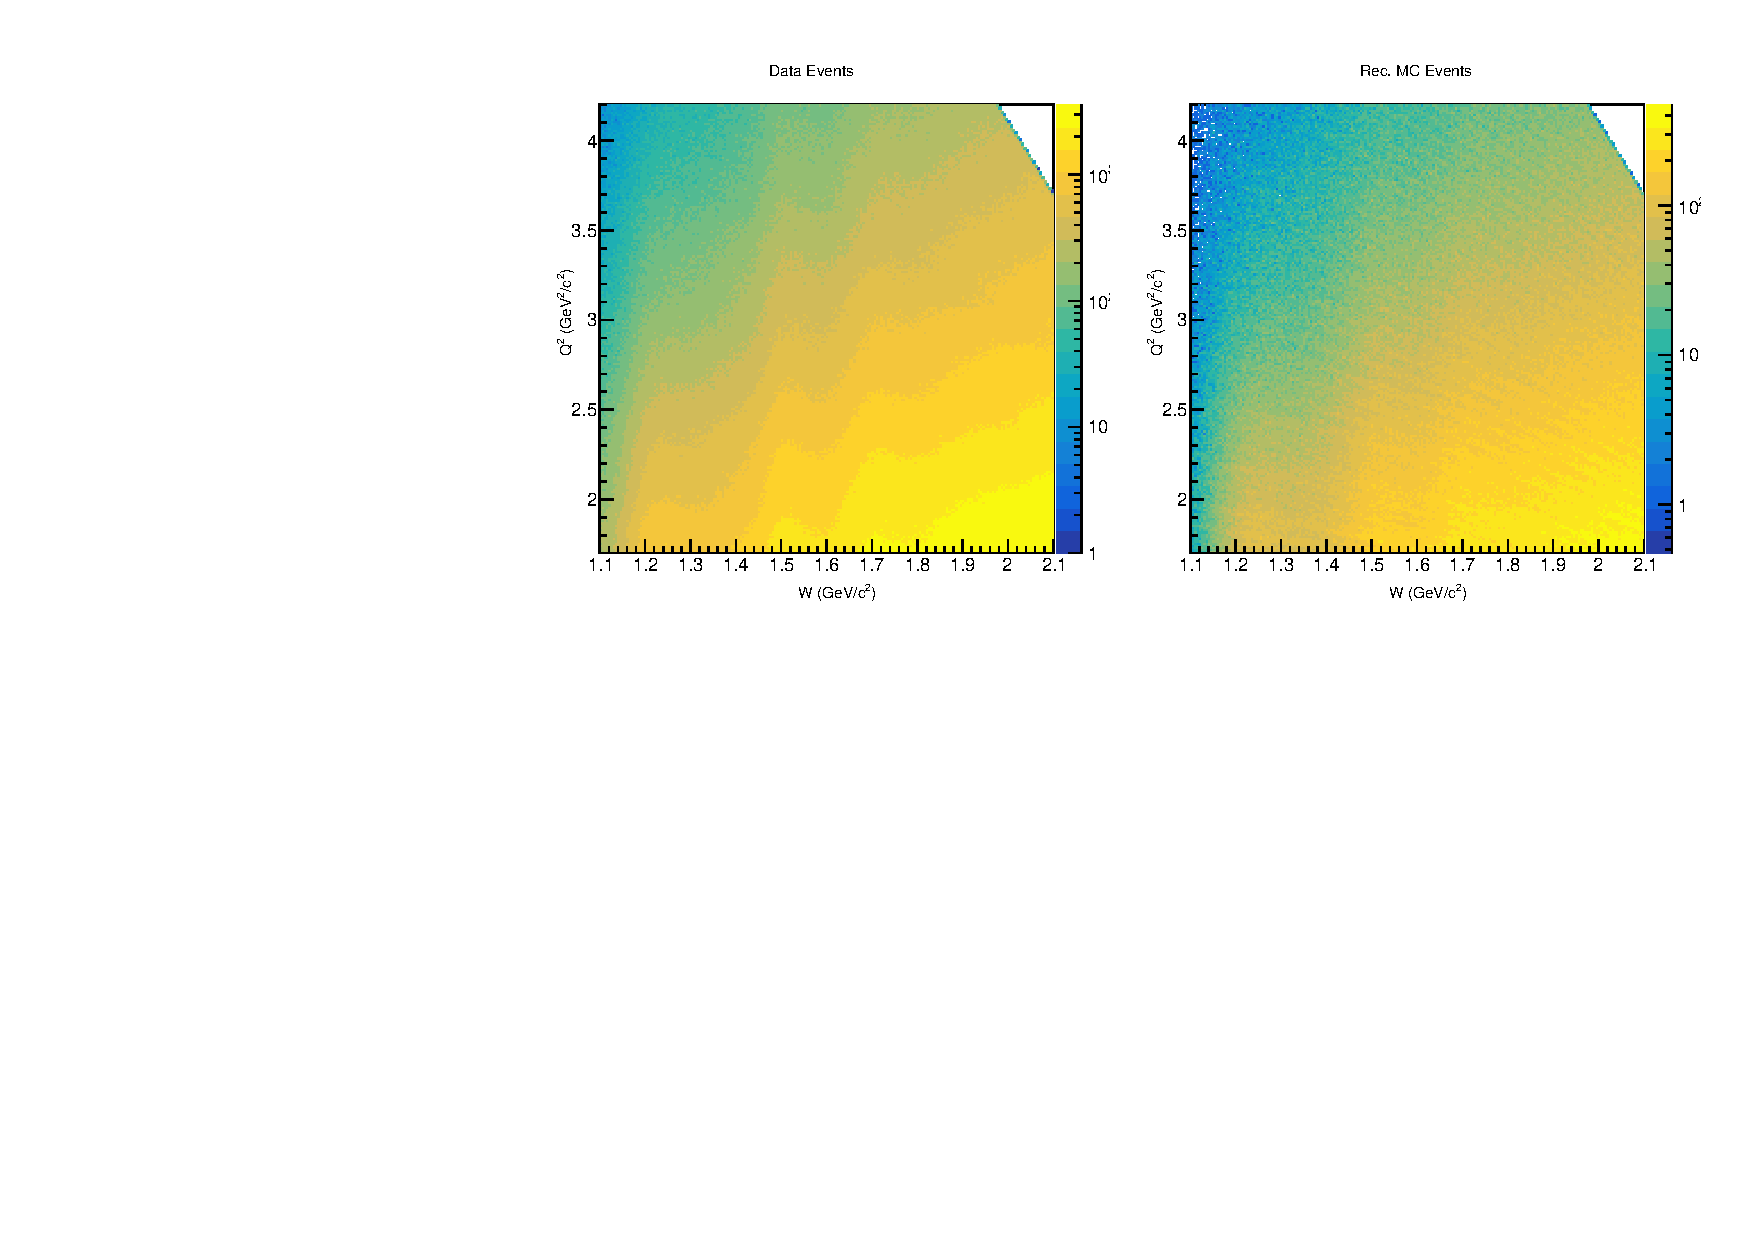
\includegraphics[width=\textwidth]{image/plots/inclusive/w_qq.pdf}
	\label{fig:wqq-data-sim}
	\caption[Inclusive data and simulation comparison.]{Data and Simulation (reconstructed) events are compared.}
\end{figure}

The problems solved by event selection are two-fold.  Typically it is required that the negative momentum transfer squared $Q^2 > 1 \; GeV^2/c^2$ is sufficiently large so that the measurement can be considered part of the DIS region.  Analyses in CLAS have typically used $1 \; GeV^2/c^2$ as the working assumption for what constitutes the lowest acceptable momentum transfer to be considered DIS, and this value is used in the SIDIS presented in this work.  Because we study the resonance region with $W \in [1.1, 2.1]$ and the beam energy is $E_{beam} = 5.498 \; GeV$ the kinematics are sparsely populated for $Q^2 < 1.6 \; GeV^2/c^2$ and this limit is applied in our study.  The second important function of event selection in this study is to avoid the largest source of background, Bethe-Heitler events. \\

As mentioned in the introduction, Bethe-Heitler events (where a real photon is radiated by the electron in the initial or final state) are the dominant source of background for this measurement.  If when studying elastic scattering the final state electron and the scattered target proton are detected, it's possible to apply energy-momentum constraints to the system and eliminate radiative Bethe-Heitler events.  However, in this measurement only the final state electron is detected and used to workout the event kinematics.  There is no way to directly apply energy-momentum converservation to eliminate Bethe-Heitler events.  Faced with this problem, we choose to restrict the values of \textit{inelasticity} $y = 1-E'/E < 0.7$ that are included in our event sample to limit this contribution.  This restriction is applied because events with large-$y$ have a significantly higher probability to be Bethe-Heitler events (this is verified by simulation and shown below in figure \ref{fig-kinematics-compare}).  This restriction is equivalent to enforcing a minimum energy for the scattered electron.

\begin{equation}
	E_{min} = E_{beam}(1-y_{max}) \approx 1.6 \; GeV  
\end{equation}   

Figure \ref{fig-kinematics-compare} shows the kinematic distribution of events from simulation and data, and illustrates the need for this $y$ cut.  The number of Bethe-Heitler events in our sample is further reduced by limiting the measurement to the resonance region.  Simulations for $E_{beam} = 5.498 \; GeV$ show that the majority of Bethe-Heitler events occur between $W \in [2, 3]$.

\begin{figure}
	\centering
	\label{fig-kinematics-compare} 
	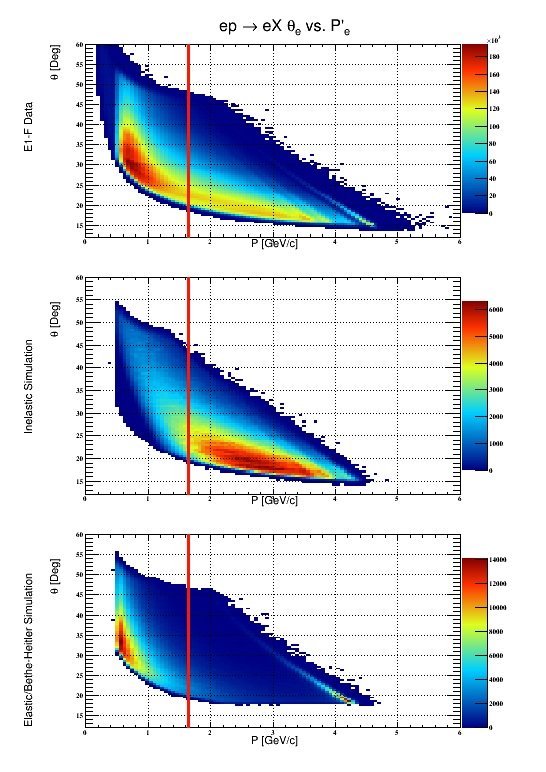
\includegraphics[width=\textwidth]{image/plots/inclusive/ycut.png}
	\caption{Event distributions ($\theta_e$ vs $p$) for data, simulated inelastic events, and simulated elastic events with radiation are shown.  The red line indicates the momentum cut applied by restricting $y < 0.7$.   The band of events on the right side of the figure contains all un-radiated elastic events.  The larger portion of events present on the left side are Bethe-Heitler events which we wish to avoid in our analysis.}
\end{figure}

\subsection{Binning}
Detected inclusive events are divided into 10 bins of equal size in $Q^2$ and 40 bins of equal size in $W$ (for a total of 400 bins for each sector).  Bins are chosen small enough in $W$ to detect resonance features, but larger than the resolution of CLAS to avoid having a large numbers of events reconstructed in a bins that they do not belong in.  Equal sized bins are chosen for their simplicity and because for cross sections (unlike asymmetry measurements) we can tolerate bins with comparatively low statistics.  The binning details are displayed in table \ref{table:bins}. 

\begin{table}
  \centering
  \begin{tabular}{c|c|c|c|c}
    Variable & N & Min. & Max & Width \\
    \hline 
    $W$   & 40 & 1.1 & 2.1 & 0.25 \\
    $Q^2$ & 10 & 1.7 & 4.2 & 0.25
  \end{tabular}
  \caption{Summary of $W$ and $Q^2$ binning used for the inclusive cross section.}
  \label{table:bins}
\end{table}

\subsection{Simulation}
All processes that CLAS measures are observed through the combination of signals from several sub-detectors.  During analysis all sub-systems are calibrated accurately, but such a complicated system still often produces distributions that do not look like the true physical distribution.  This discrepancy arises from the combination of several effects.

\begin{enumerate}
	\item Holes, barriers, obstructions, shadows of other detectors, and any other physical effects that prevent events from being measured in some range of $\theta, \phi$ are known as geometrical acceptance effects.  An important geometrical acceptance effect is the presence of the torus coils in between every sector.  These represent a complete loss of information for a small range of $\phi$ between each sector.
	\item Inefficiencies due to the probabalistic nature of particle interaction in the detector subsystems.
	\item Detectors have finite spatio-temporal resolutions.  
\end{enumerate}

In order to understand and limit the impact of these effects on the physics extracted from the experiment, a mock experiment is simulated.  In the simulated experiment everything is modeled as realistically as possible.  The simulation used for CLAS is called GSIM and is based on the CERN package GEANT3 (GEometry ANd Tracking).\\
In this controlled environment, samples of events can be generated and fed into the simulation.  The output of GSIM is a bos file that is similar to the raw data from the data acquisition system. This is then reconstructed using the same reconstruction algorithm that is applied to data (\texttt{userana}).  \\ 

\subsection{Acceptance Corrections (Theory)}
By retaining the truth information for all particles that are generated, the effect of the detector can be studied completely.  These concepts can be stated more formally by considering the true $t(x')$ and measured $m(x)$ distributions of some observable.  In the absence of background processes, the relationship between these distributions is expressed as a Fredholm integral equation of the first kind.

\begin{equation}
	m(x) = \int_{\Omega} K(x,x') t(x') dx'
\end{equation}
    
Here $K(x,x')$ is a kernel which encodes information about detector acceptance due to the effects described above.  The goal of the Monte Carlo simulation is to \textit{unfold} the measured distribution $m(x)$ by providing an estimate of $K(x,x')$ and finally corrected the data to get $t(x)$.\\
Observed events are usually aggregated into bins and the problem is naturally discretized and written in vector-matrix form.

\begin{equation}
	\mathbf{A} \mathbf{x} = \mathbf{y}
\end{equation}        

In this notation $\mathbf{A}$ represents the response matrix, a discretized version of the kernel function $K$, the vector $\mathbf{y}$ represents the measured distribution in the bins, and the vector $\mathbf{x}$ is the true distribution over the bins.  The matrix elements $A_{ij}$ can be estimated by using generating events, passing them through a Monte-Carlo detector simulation, and then counting the number of events that are reconstructed in bin $i$ when generated in bin $j$.  This quantity is then normalized by the total number of events generated in the $j^{th}$ bin.  In the absence of bin migration and with perfect acceptance this matrix is the identity matrix $I^{n}$ where $n$ is the total number of bins. \\

\begin{equation}
  A_{ij} = \frac{n_{rec=i, gen=j}}{n_{gen=j}}
\end{equation}

The binned true distribution can be recovered by inverting the response matrix and correcting the observed distribution.

\begin{equation}
  \mathbf{x} = \mathbf{A}^{-1} \mathbf{y} 
\end{equation}

In the absence of bin migration, the matrix becomes diagonal with efficiency elements $\epsilon_i$ that represent the fraction of events reconstructed in the bin $i$.

\begin{equation}
  \mathbf{A} = \begin{pmatrix}
    \epsilon_0 & 0 & 0\\
    \vdots & \ddots \\
    0 &  & \epsilon_n \\
  \end{pmatrix}
\end{equation}


The inverse is, 
\begin{equation}
  \mathbf{A}^{-1} = \begin{pmatrix}
    1/\epsilon_0 & 0 & 0\\
    \vdots & \ddots \\
    0 &  & 1/\epsilon_n \\
  \end{pmatrix}
\end{equation}

and the corrected observation for the $i^{th}$ bin is simply given by the observation over the efficiency.

\begin{equation}
  t_i = \frac{m_i}{\epsilon_i} = m_i \frac{n_{gen=i}}{n_{rec=i}}
\end{equation}

This is the simple \textit{bin-by-bin} acceptance correction method, which is widely used and produces accurate results provided that bin migration is not significant.  In this analysis the simple bin-by-bin acceptance correction is used.  

\subsection{Acceptance Corrections}
\begin{sidewaysfigure}
	\centering
	\label{fig-rec-events} 
	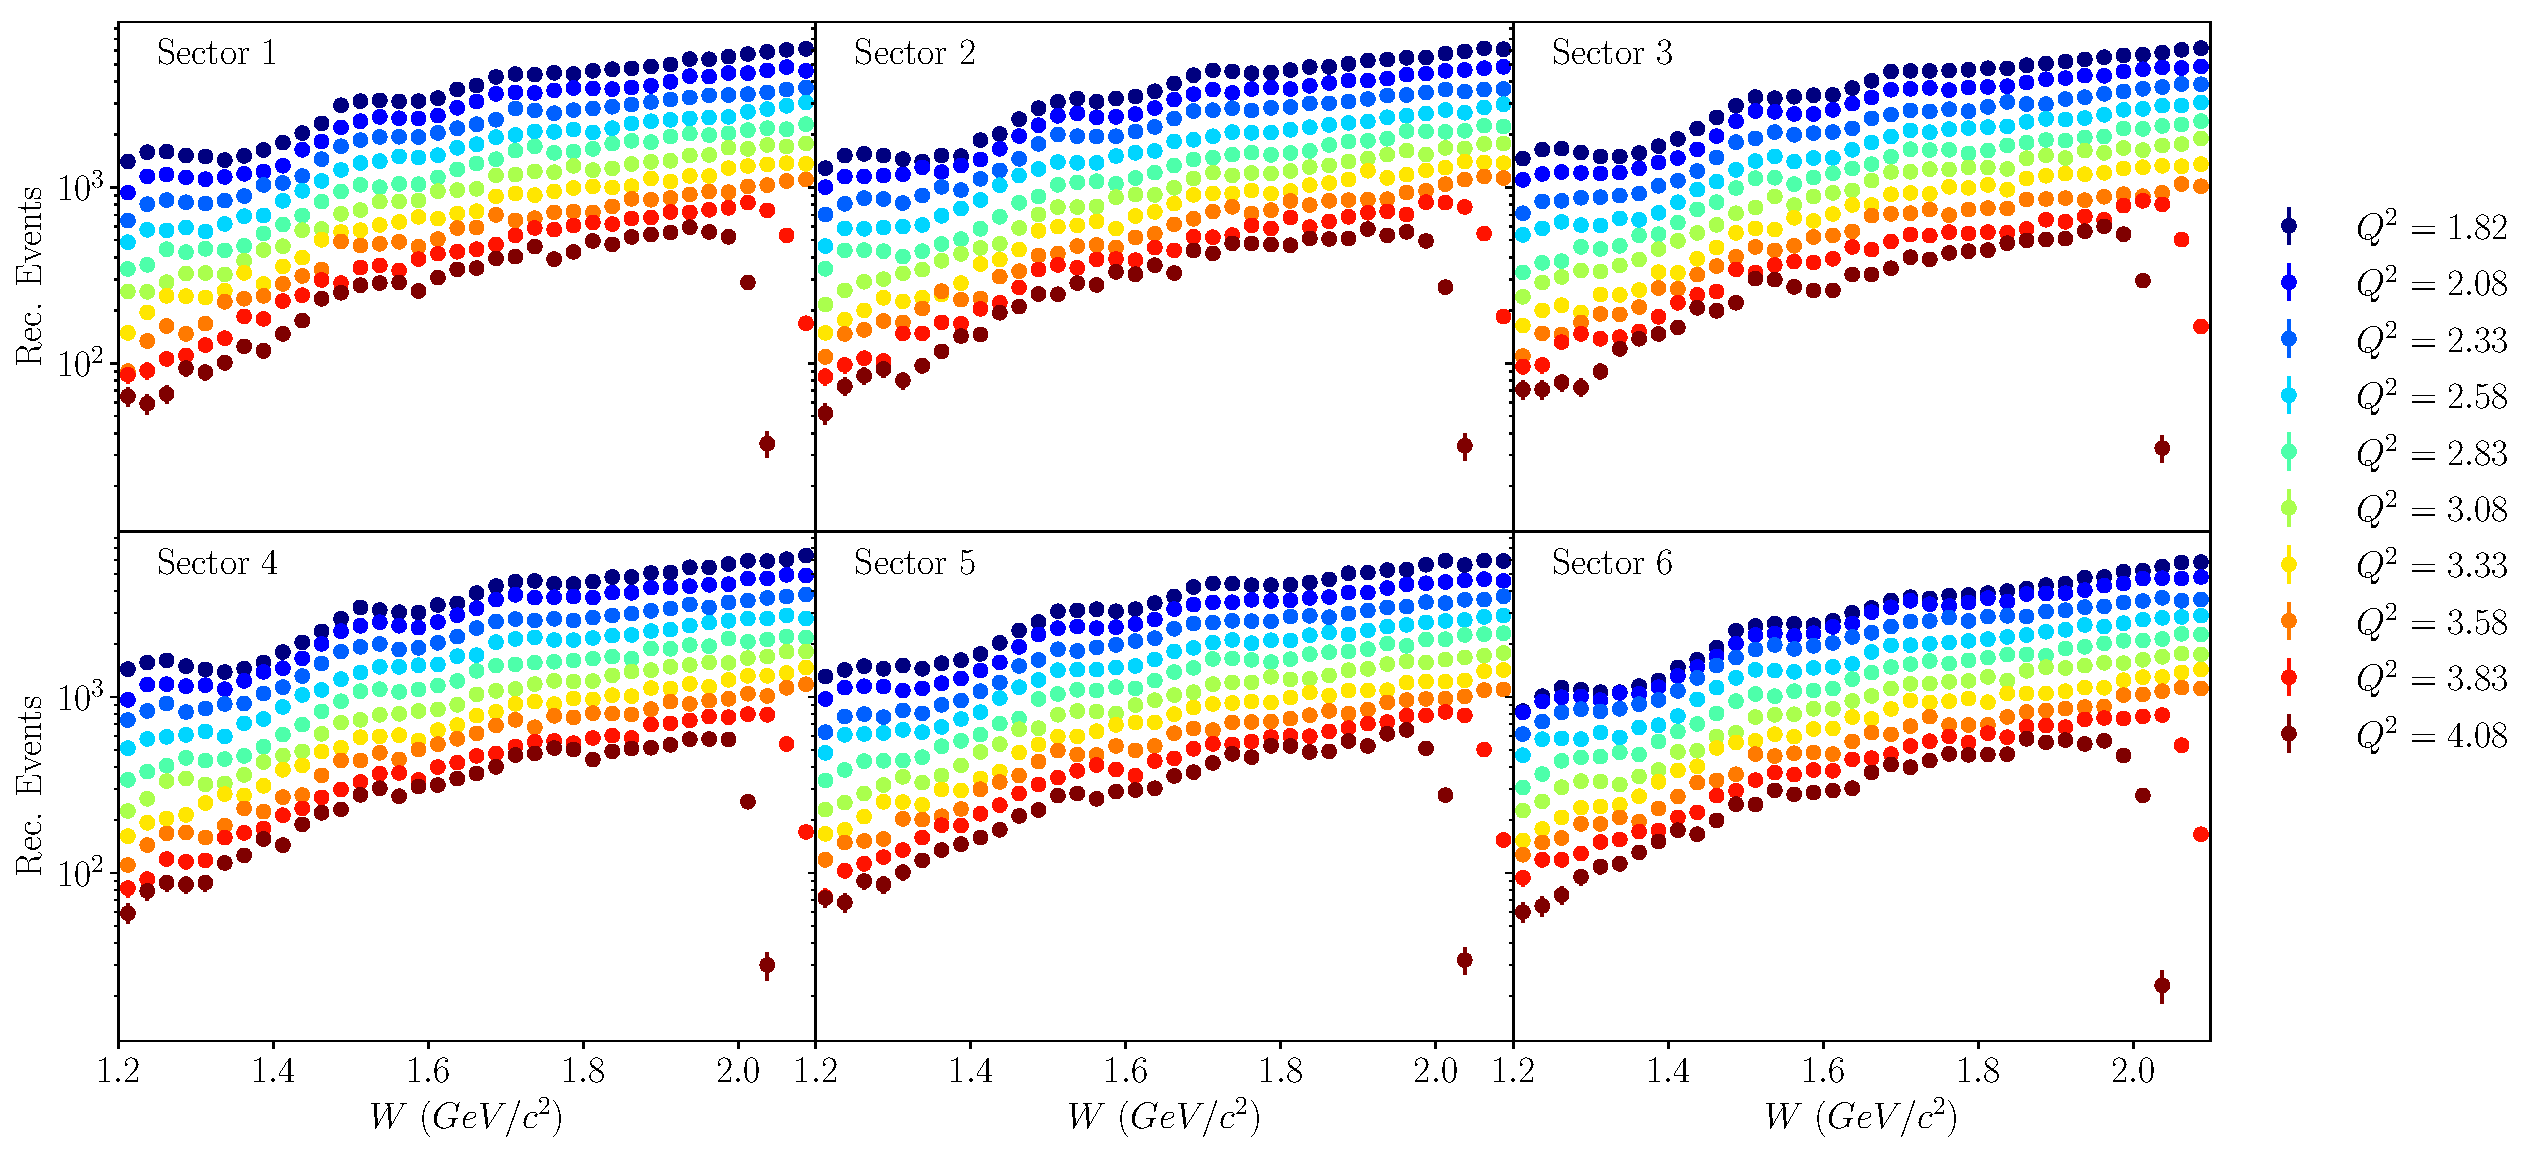
\includegraphics[width=\textwidth]{image/plots/inclusive/rec_events_superimposed.pdf}
	\caption{Reconstructed Monte Carlo events displayed for different sectors (by panel) and different $Q^2$ bins represented by different colors.}
\end{sidewaysfigure}

\begin{sidewaysfigure}
	\centering
	\label{fig-gen-events} 
	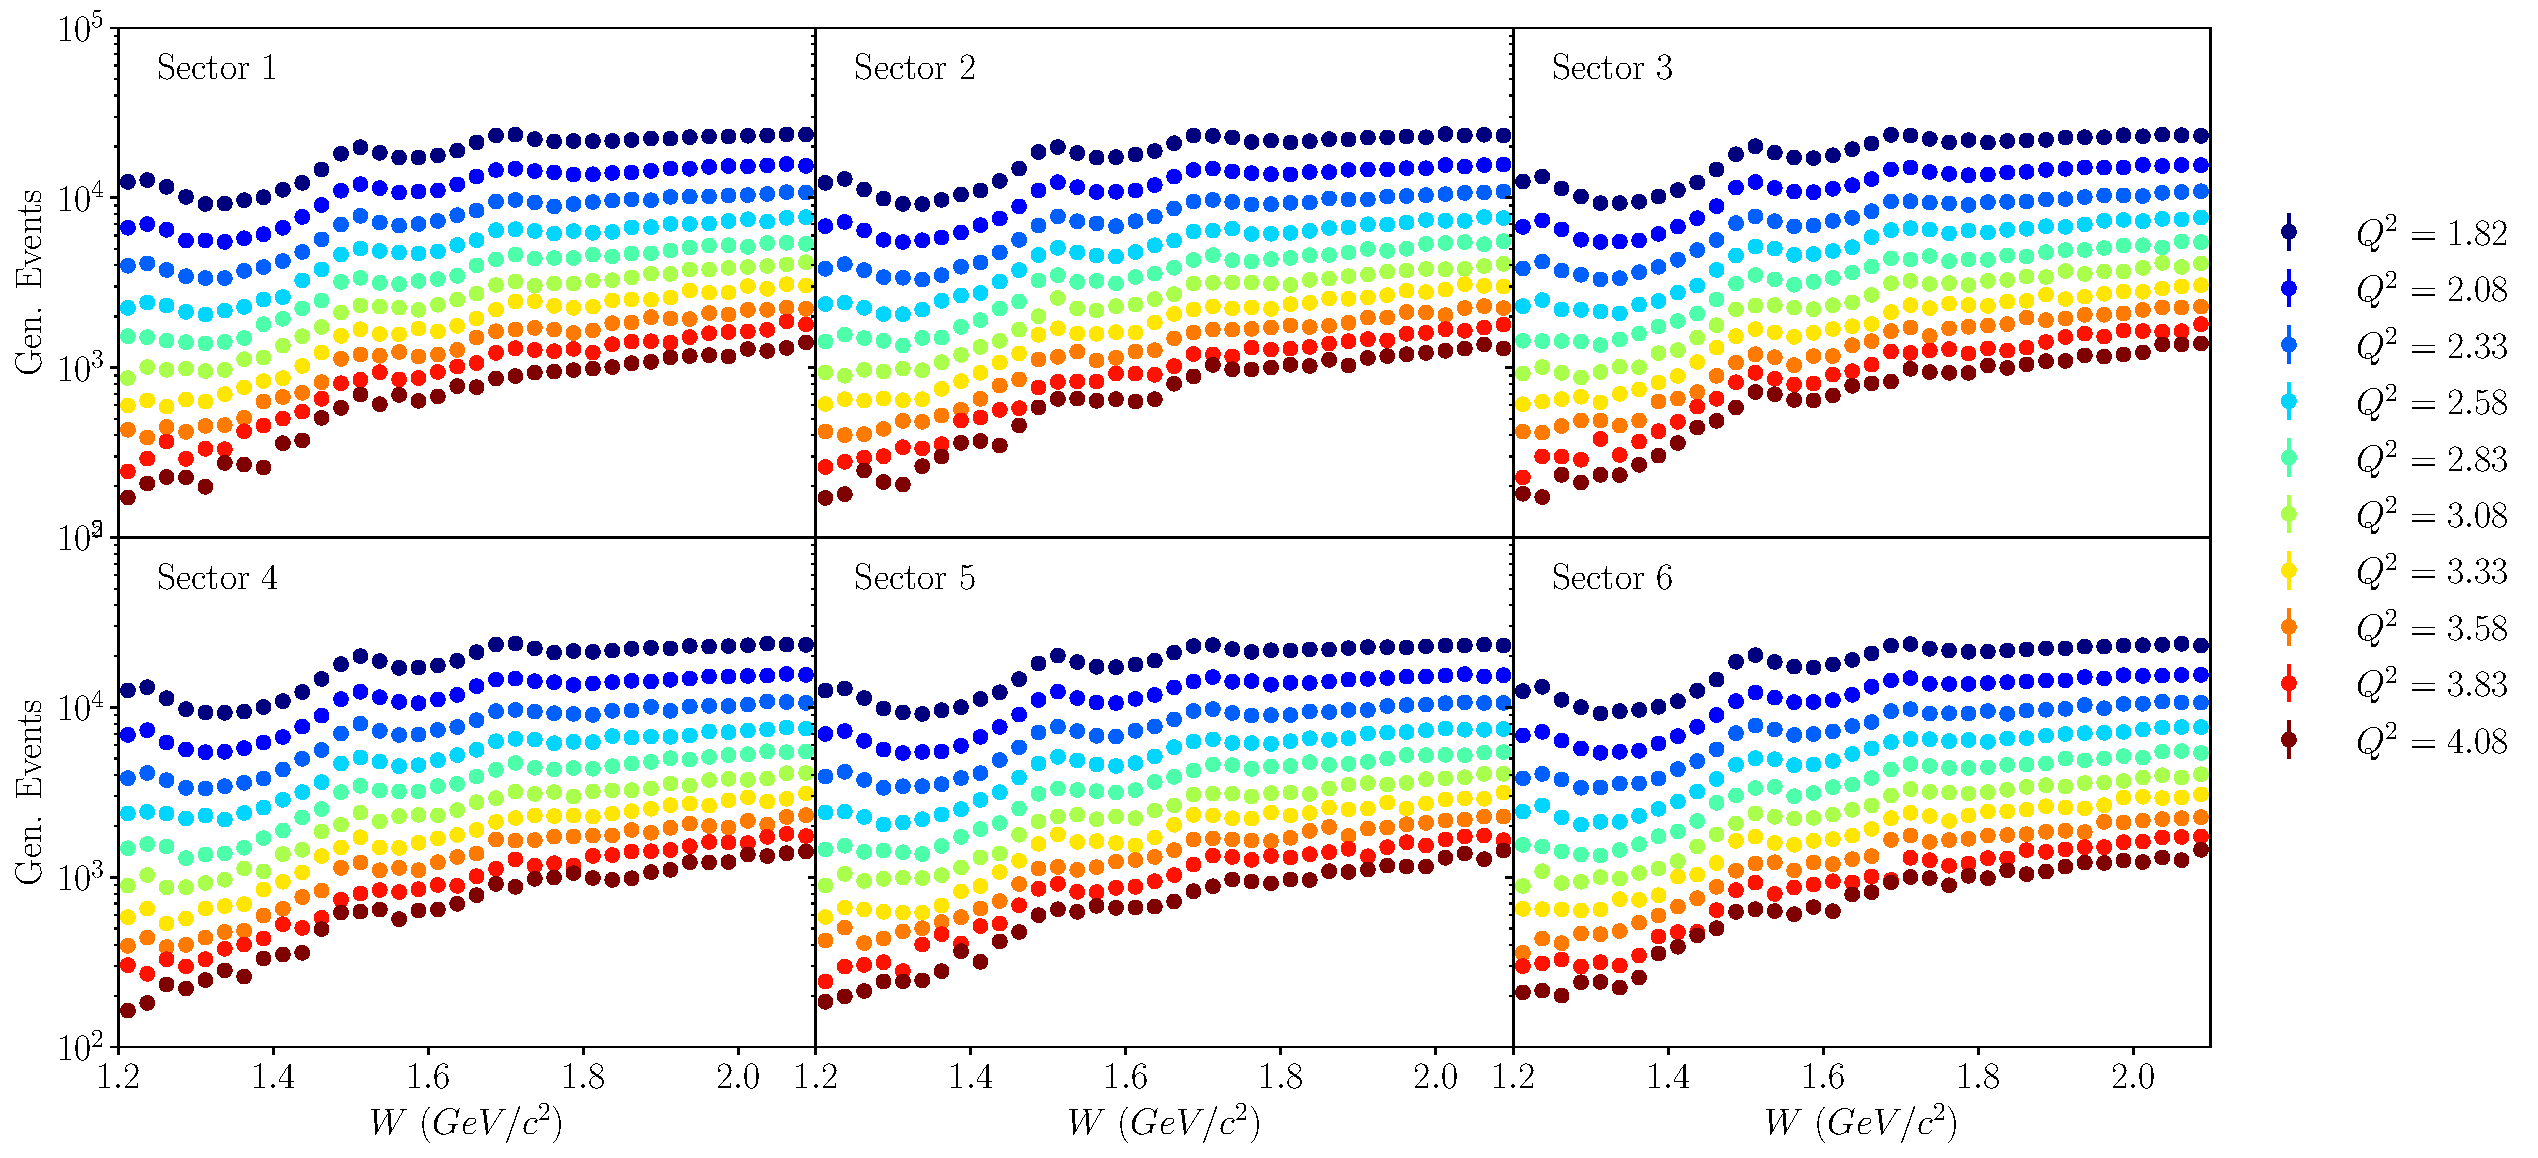
\includegraphics[width=\textwidth]{image/plots/inclusive/gen_events_superimposed.pdf}
	\caption{Generated Monte Carlo events displayed for different sectors (by panel) and different $Q^2$ bins represented by different colors.  These events were generated with radiative effects.}
\end{sidewaysfigure}

\begin{sidewaysfigure}
	\centering
	\label{fig-data-rec-grid} 
	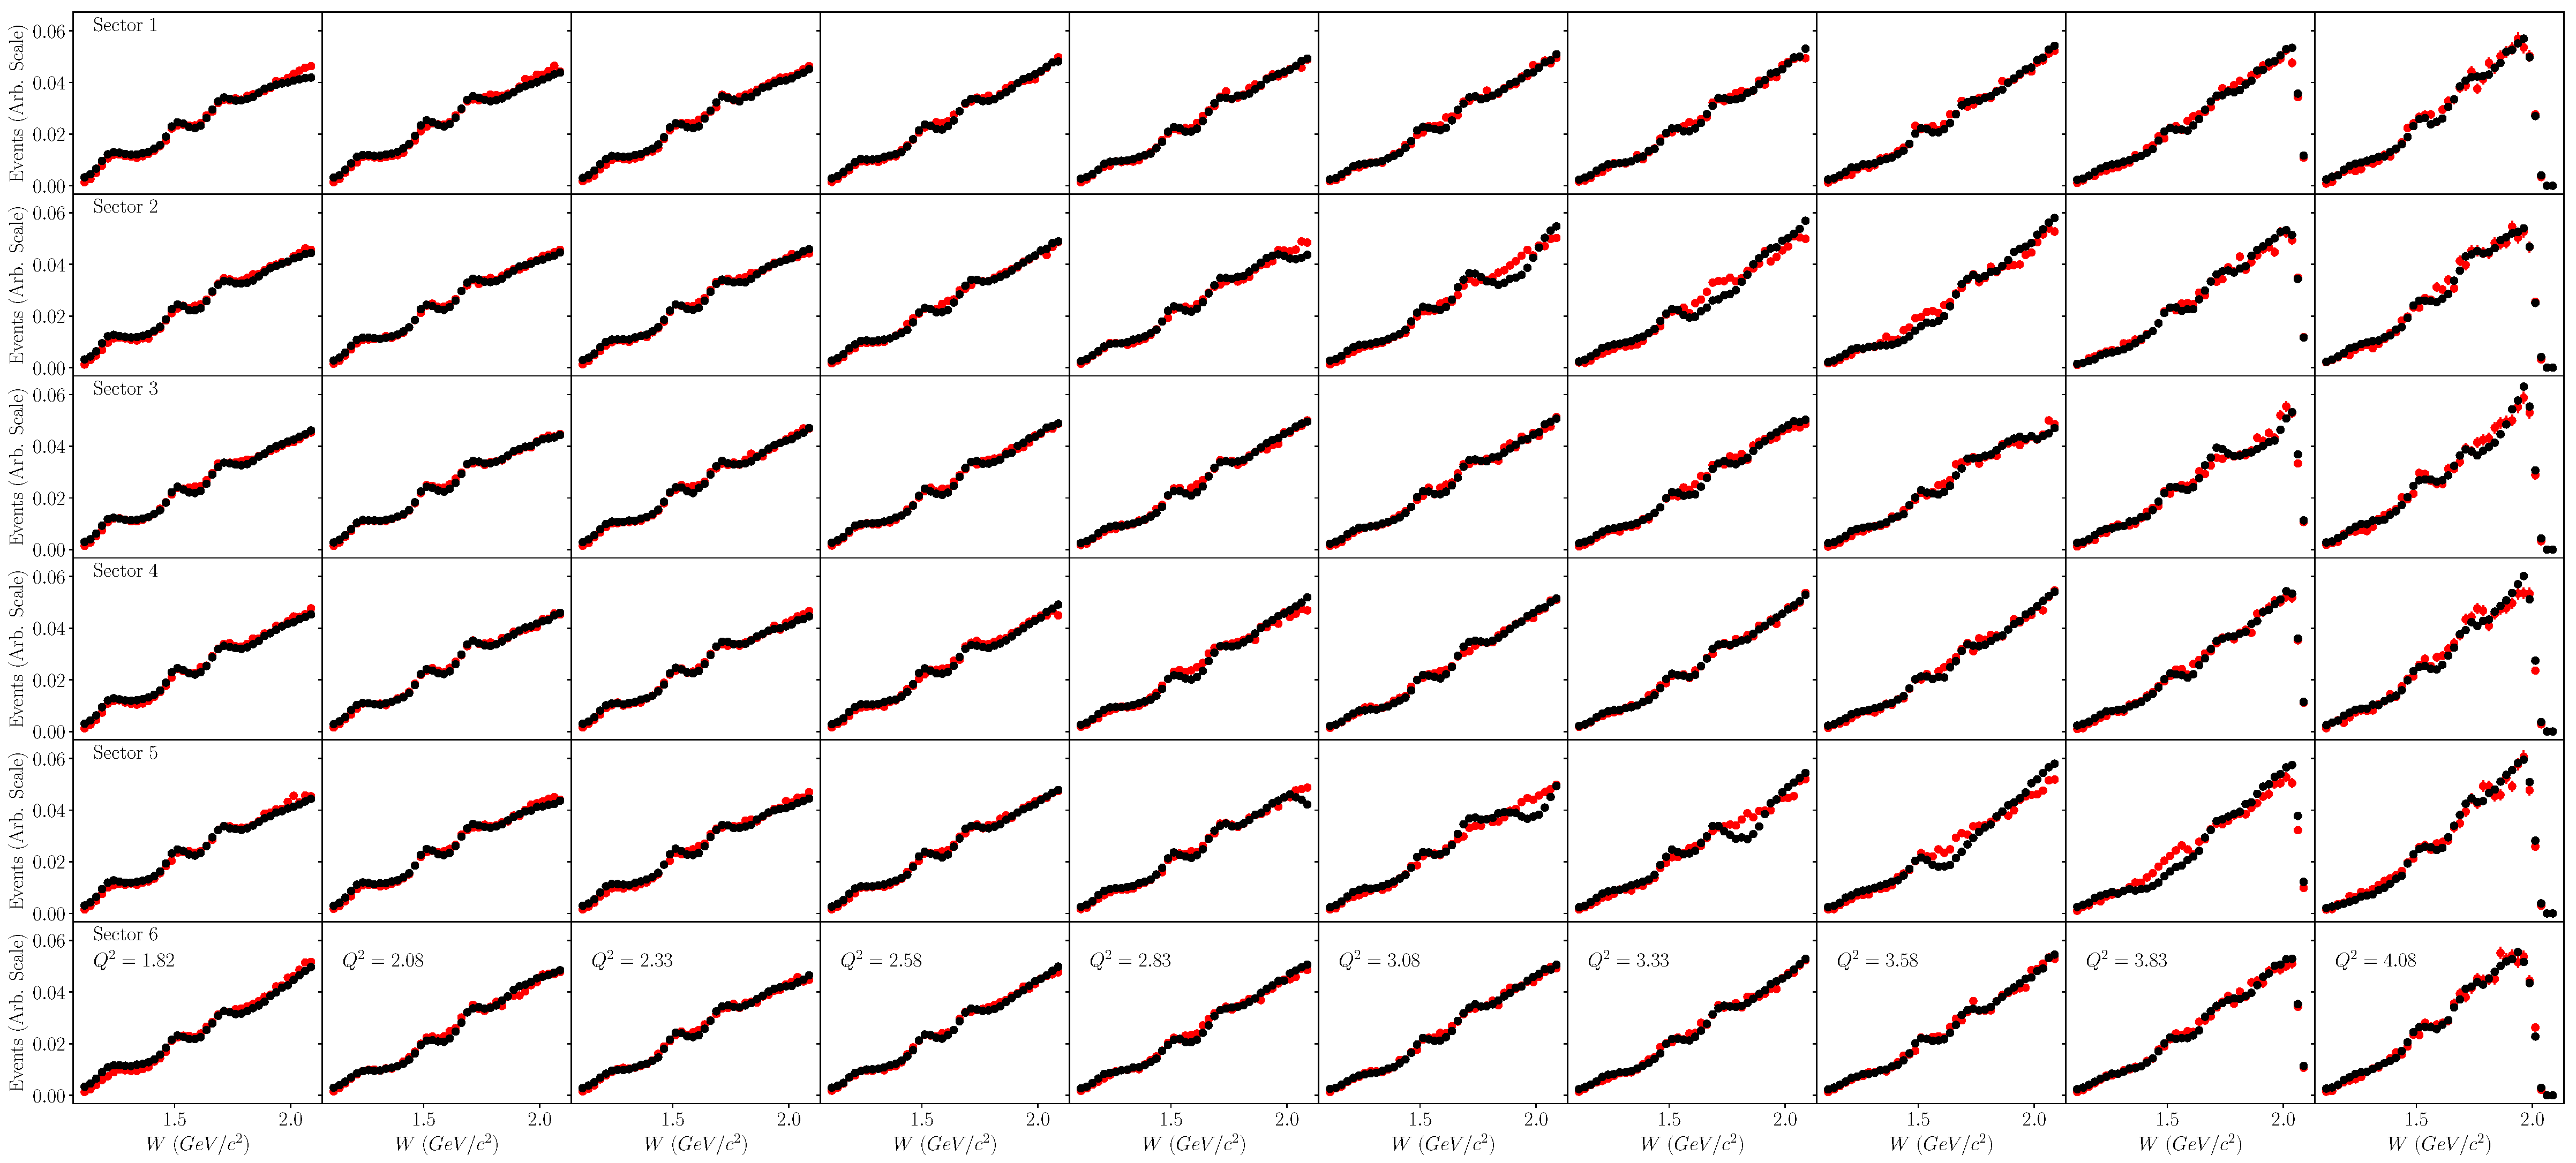
\includegraphics[width=\textwidth]{image/plots/inclusive/compare_data_rec_grid.pdf}
	\caption{Reconstructed events from data (black) and Monte Carlo (red) are superimposed to show that the simulation is a good approximation to the physics, a fact important for the accurate calculation of acceptance.}
\end{sidewaysfigure}

\begin{sidewaysfigure}
	\centering
	\label{fig-acceptance-grid} 
	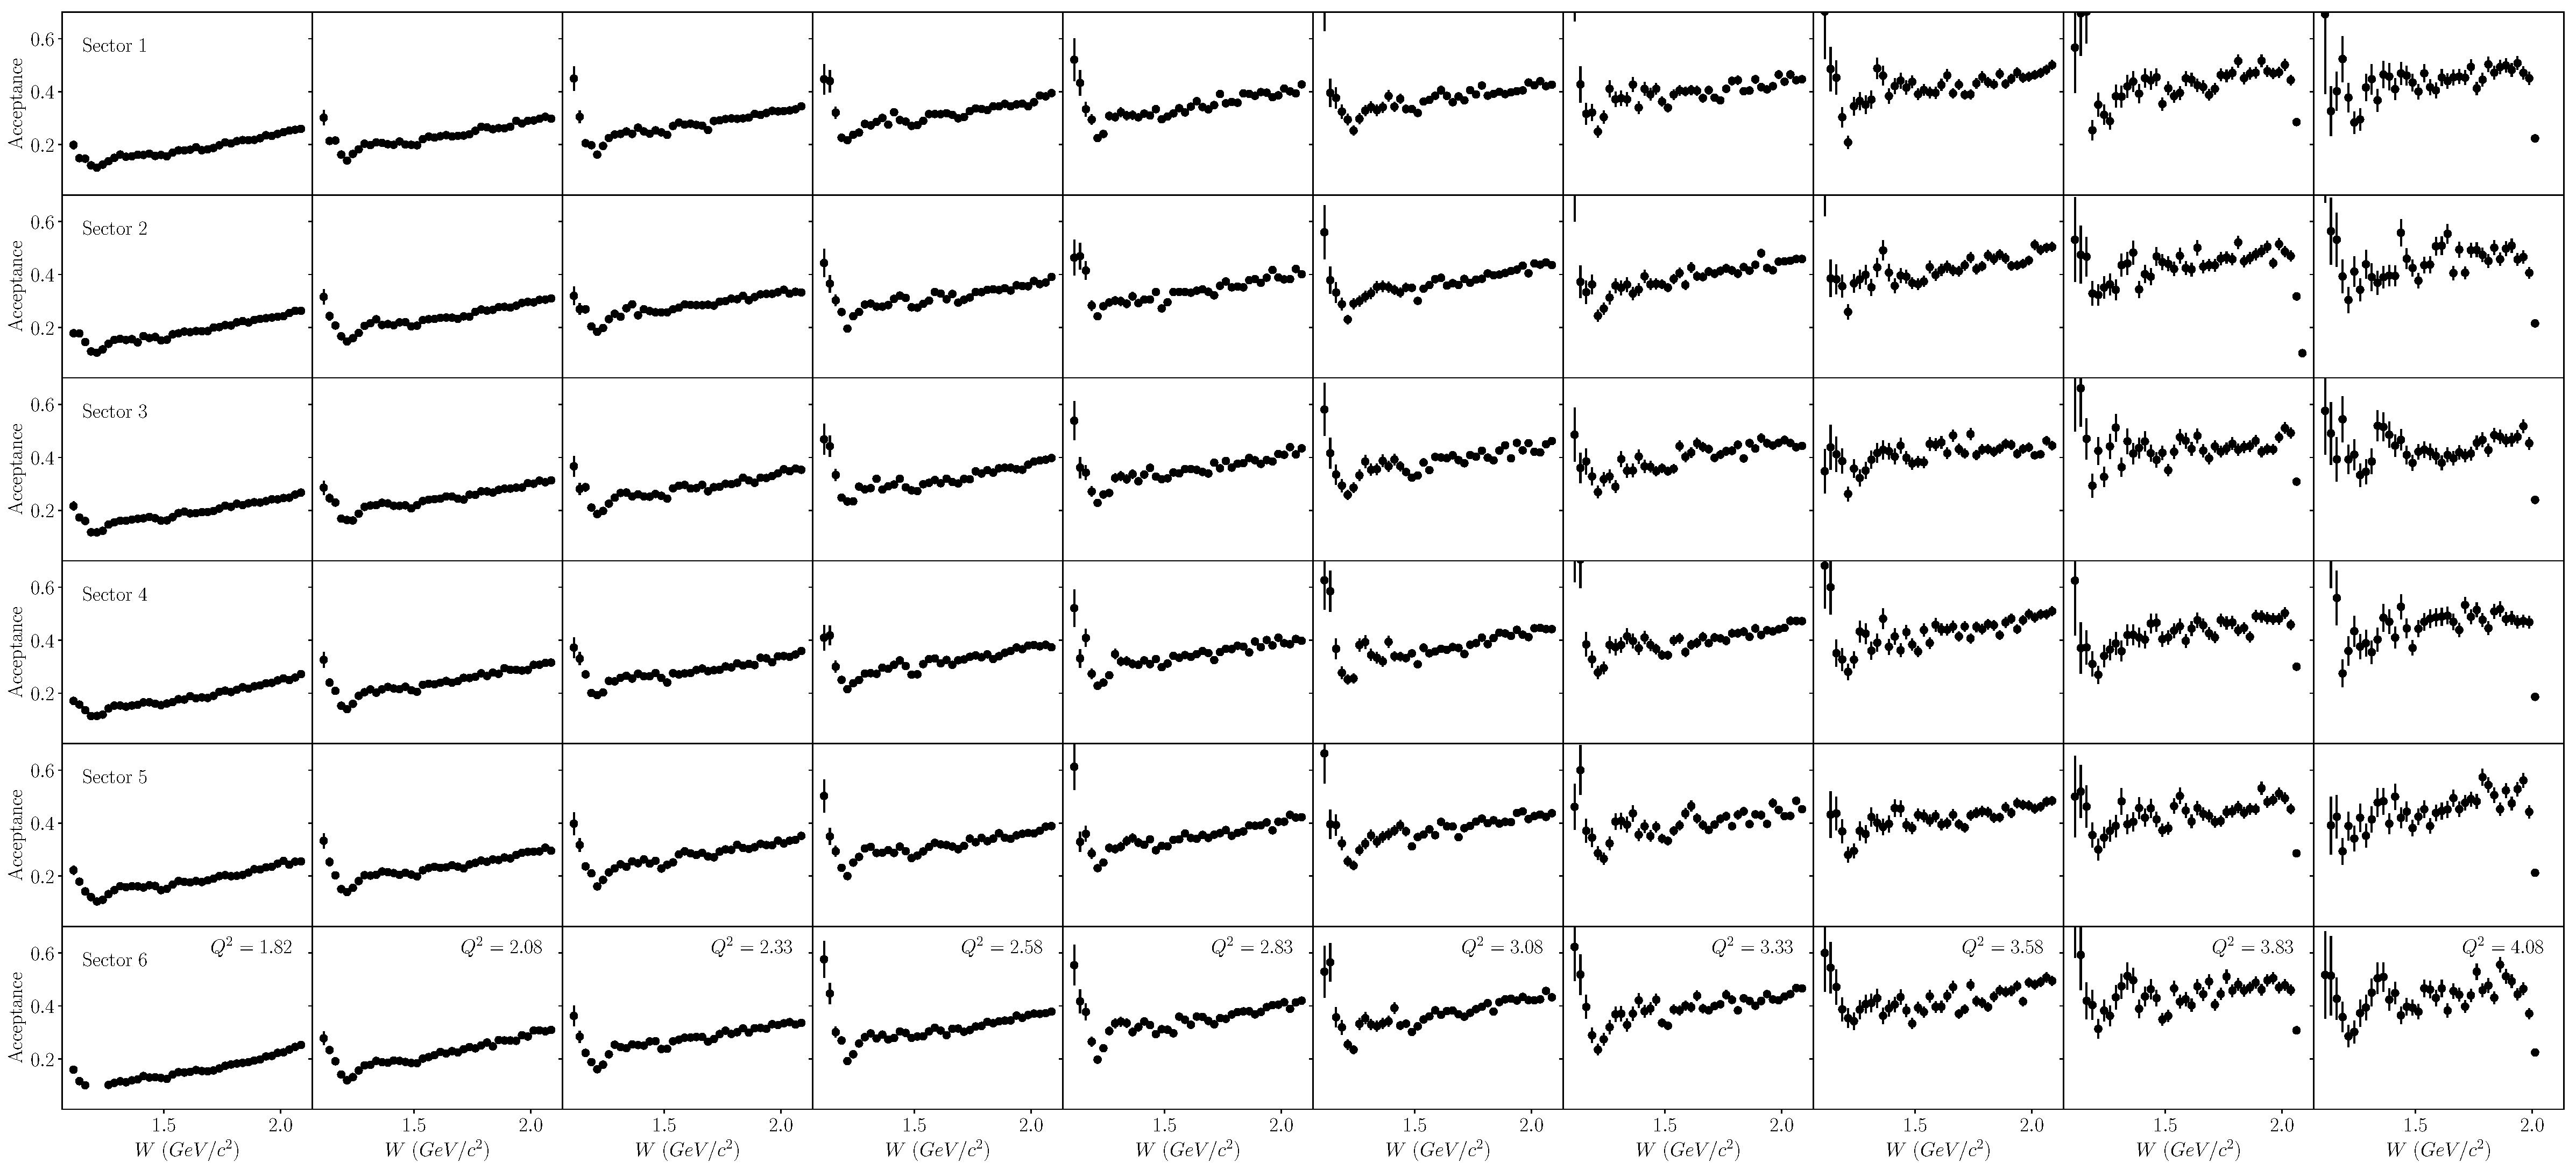
\includegraphics[width=\textwidth]{image/plots/inclusive/acceptance_grid.pdf}
	\caption{Acceptance corrections applied to the inclusive cross section are shown above in sixty panels that correspond to increasing $Q^2$ from left to right, and increasing sector number from top to bottom.  }
\end{sidewaysfigure}

\subsection{Radiative Corrections}

Inclusive events detected in CLAS are really \textit{radiated} inclusive events.  By using the term \textit{radiated}, one implies that the electron could have radiated a real photon in the initial or final state, or that internal radiative correction diagrams could have influenced the event kinematics.  Unfortunately, there is no way of differentiating these events.  For this reason, a radiative correction procedure that unfolds these effects from the cross section is applied to our measured distributions.  \\

Two Monte Carlo event generators are used to calculate radiative corrections for each bin, both sample from the cross section model discussed in the beginning of the chapter.  The first program generated events with no radiative corrections by sampling directly from the cross section model.  The second program uses the same cross section model but generates radiated events following the procedure of Mo and Tsai \cite{misc-mo:1969} which includes corrections due to internal and external Bremsstrahlung.  The correction ratio for the $i^{th}$ bin $R^{(i)}$ is defined for the $i^{th}$ bin as shown below. 

\begin{equation}
  R^{(i)} = \frac{n_{unrad}^{(i)}}{n_{rad}^{(i)}}
\end{equation}

This factor can be estimated without passing events through the simulation (this is true if the acceptance is the same for both models, an assumption which is only invalid if the models are appreciably different) and the results are used directly from the output of the event generator to correct the cross section.  

\begin{sidewaysfigure}
	\centering
	\label{fig-rad-corr-grid} 
	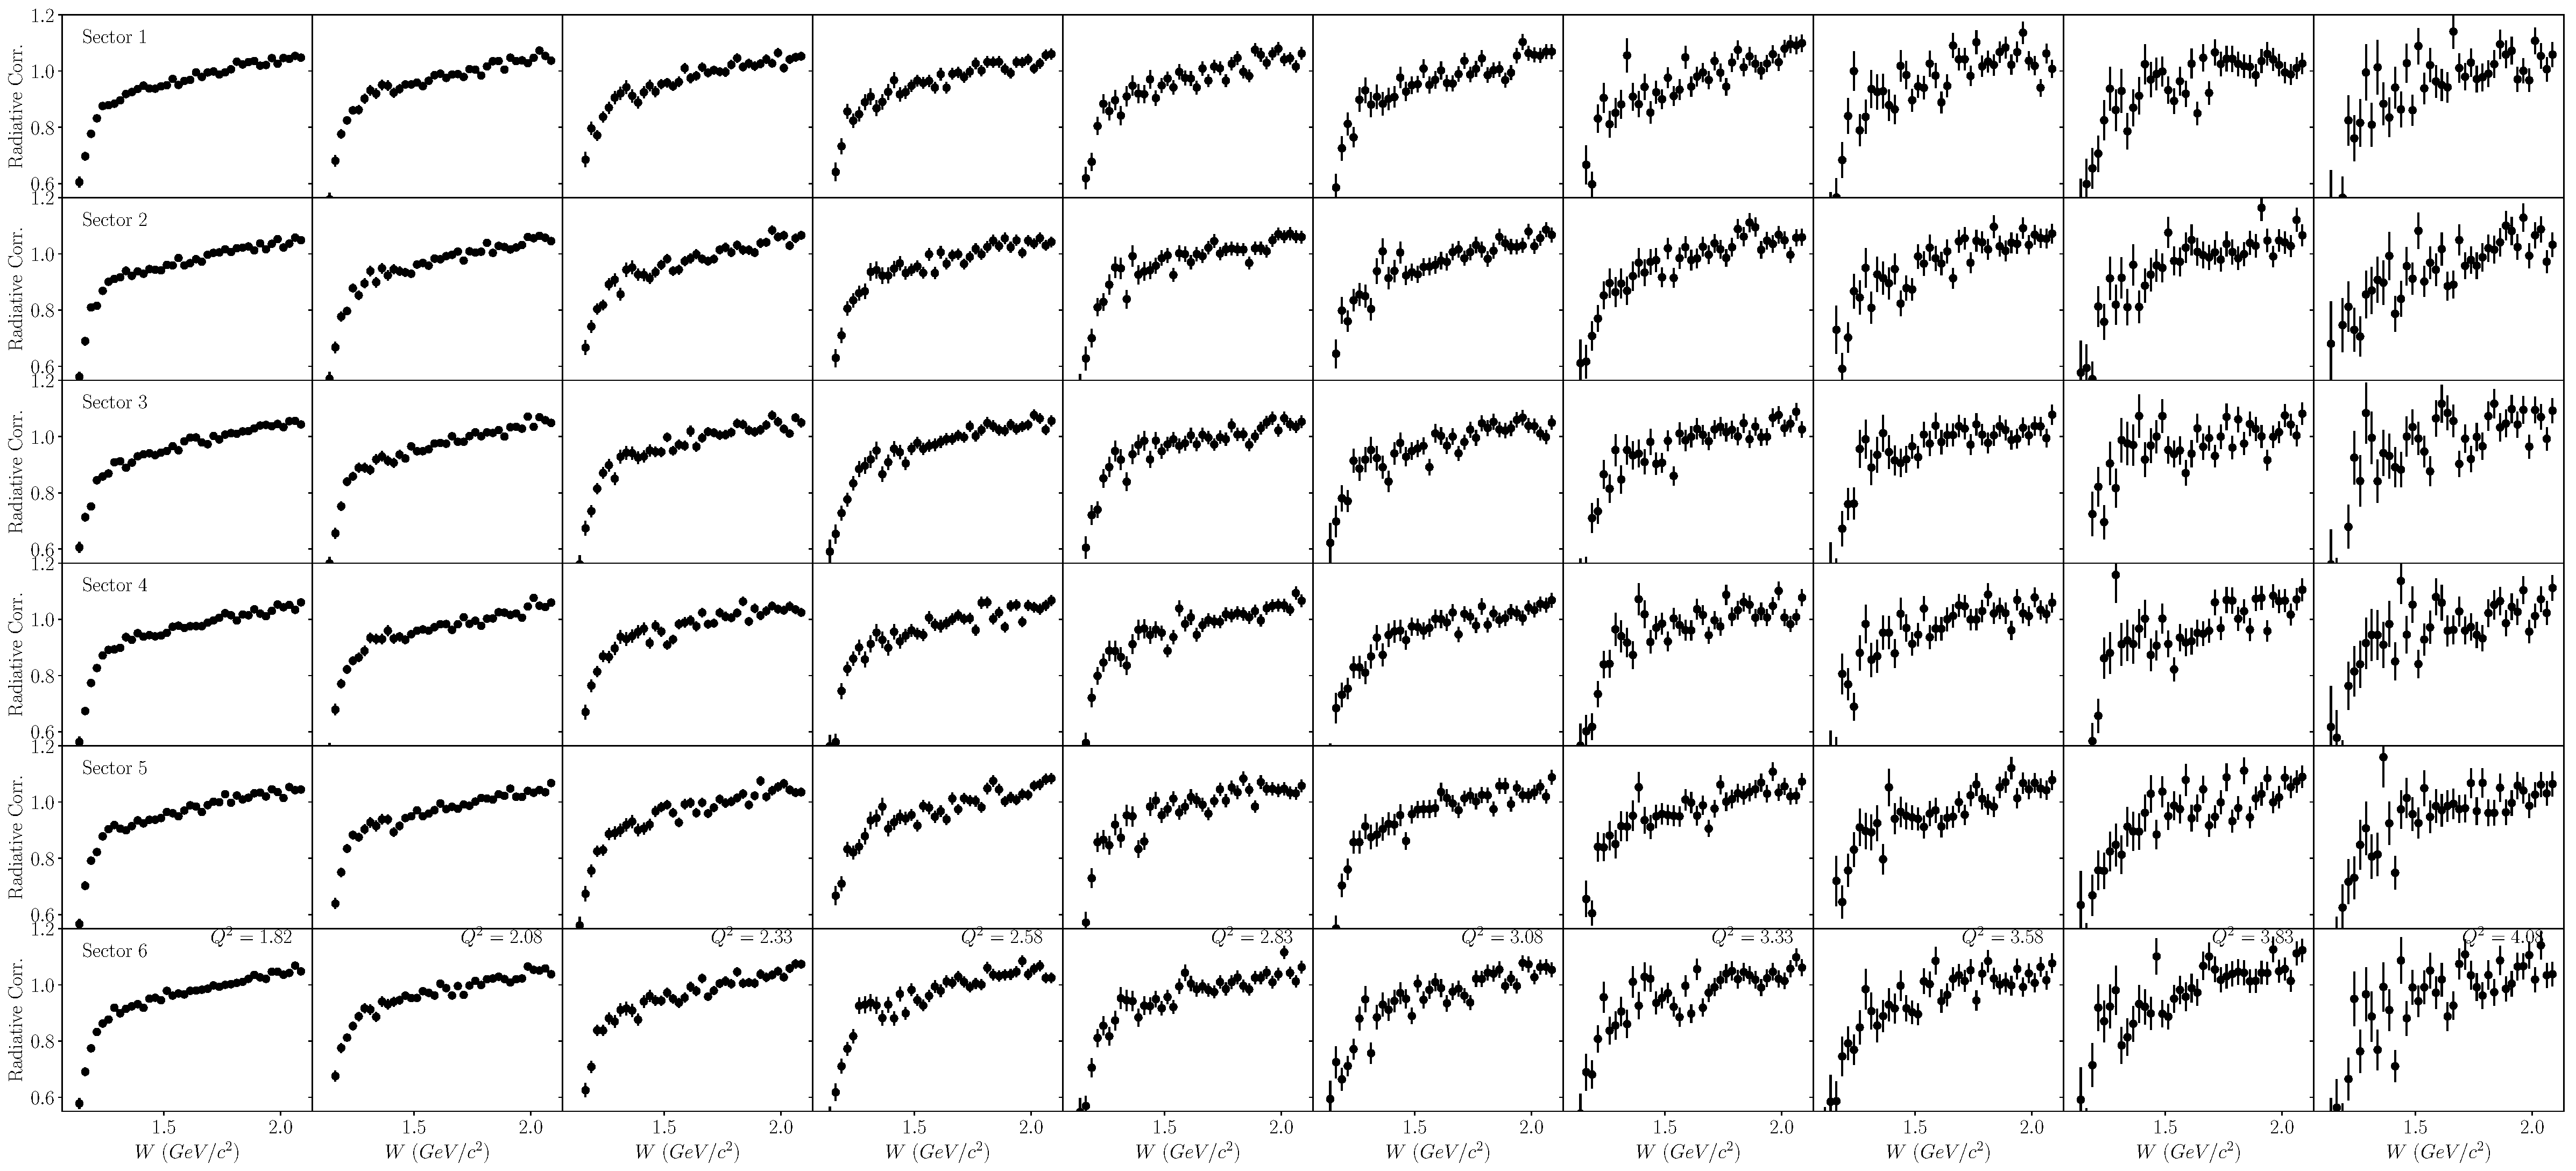
\includegraphics[width=\textwidth]{image/plots/inclusive/rad_corr_grid.pdf}
	\caption{Radiative corrections applied to the inclusive cross section are shown above in sixty panels that correspond to increasing $Q^2$ from left to right, and increasing sector number from top to bottom.  }
\end{sidewaysfigure}

\subsection{Bin Center Corrections}
Measurement of the cross section is done in bins, meaning that what is actually measured is the average cross section over some finite range of $W$ and $Q^2$ for each bin.  When reporting and plotting the results the $W$ and $Q^2$ value at the center of the bin is typically quoted.  If a model is available for comparison, the model is usually queried at the bin center, and the resulting prediction is often incorrect.  In order to obtain the correct prediction, one should average the model prediction over the measured bin.  In this study, an accurate model prediction is available (described in detail below) and a correction factor is applied to the measured cross section value to remove the effect of plotting and reporting the cross section at the central bin value.  The factor, 

\begin{equation}
	B_{i} = \frac{\sigma_{center}}{\sigma_{avg}}
\end{equation}

$B_i$ is calculated from the model for each bin $i$ and applied to the measured cross section.  This factor is calculated once for each bin, and does not depend on the sector.  We observe that the correction factor depends more strongly on $Q^2$ than $W$ which is sensible because the cross section varies more rapidly over $Q^2$.  Additionally, the correction factor is larger near the resonances in $W$.

\begin{figure}
	\centering
	\label{fig-bin-centering-correction} 
	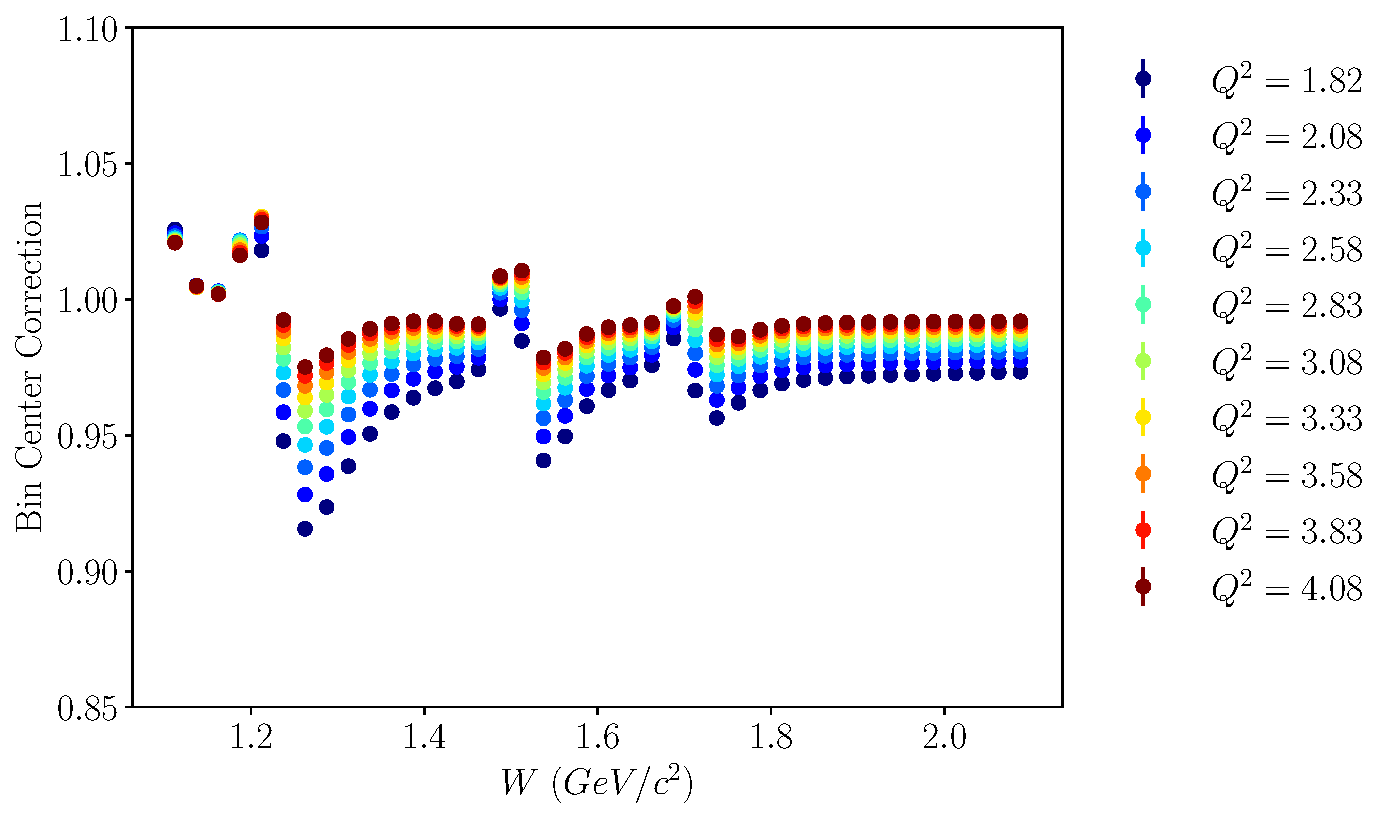
\includegraphics[width=14cm]{image/plots/inclusive/bin_center_correction.pdf}
	\caption{The bin center correction applied to the inclusive cross section is shown for different values of $Q^2$ (indicated by color) as a function of $W$ on the horizontal axis.   This correction is the same for all sectors.}
\end{figure}

\subsection{Model Comparison}

\begin{sidewaysfigure}
	\centering
	\label{fig-inclusive-xs} 
	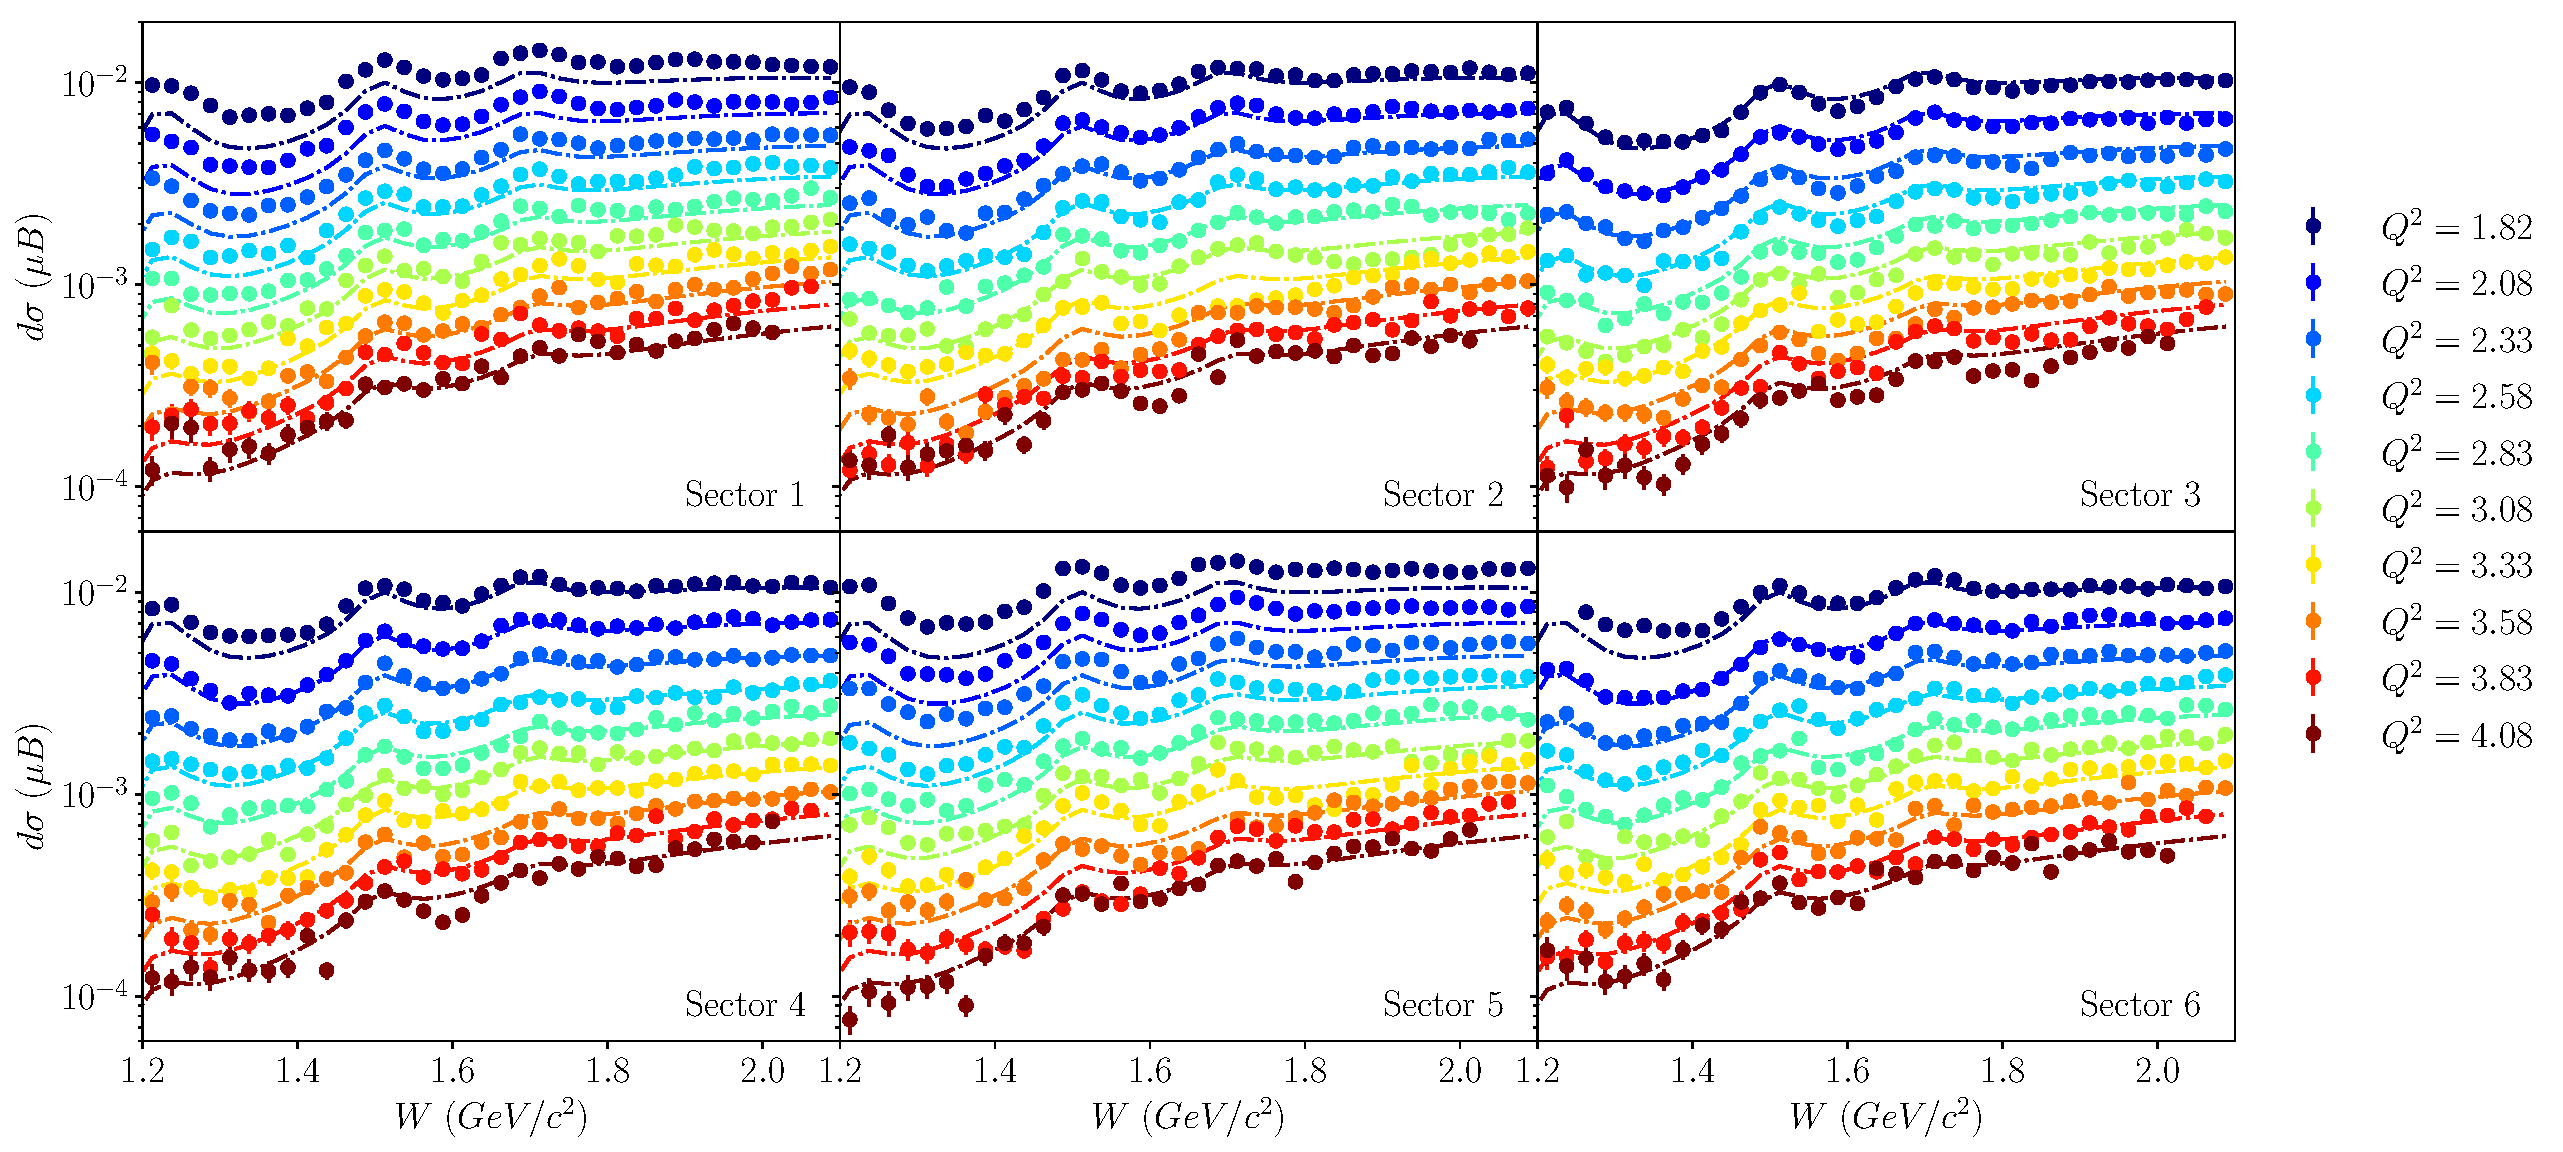
\includegraphics[width=\textwidth]{image/plots/inclusive/inclusive_xs.pdf}
	\caption{Each panel above shows one of the six sectors of CLAS, the horizontal axis shows $W$ and superimposed on the figure are the cross sections for different bins of $Q^2$.  For simplicity of the visualization each reported value of $Q^2$ is the bin center.}
\end{sidewaysfigure}

The cross section extracted in this study is in agreement with the predictions from the model, shown in figure \ref{fig-inclusive-xs}.  


